\documentclass[11pt,letterpaper]{article}
\usepackage[T1]{fontenc}
\usepackage[scaled]{helvet}
\renewcommand{\familydefault}{\sfdefault}
\usepackage{amsmath,amssymb}
\usepackage[margin=0.8in,bottom=0.9in]{geometry}
\usepackage[most]{tcolorbox}
\usepackage{tikz}
\usetikzlibrary{calc}
\usepackage{enumitem}
\usepackage{array}
\usepackage{needspace}
\usepackage{fancyhdr}
\usepackage{pifont}

% ---- Palette "F. Bright & Playful" ----
\definecolor{fmtitle}{HTML}{3D2C8D}
\definecolor{fmkey}{HTML}{0096C7}
\definecolor{fmwatch}{HTML}{2BB673}
\definecolor{fmturn}{HTML}{F4A100}
\definecolor{fmmistake}{HTML}{EF476F}
\definecolor{fmnotice}{HTML}{9B5DE5}
\definecolor{fmgray}{HTML}{6B6B6B}

\pagestyle{fancy}
\fancyhf{}
\renewcommand{\headrulewidth}{0pt}
\fancyfoot[C]{\footnotesize\color{fmgray}\textcopyright\ 2026 FangMath. All rights reserved.}
\fancyfoot[R]{\footnotesize\color{fmgray}\thepage}
\setlength{\parindent}{0pt}
\setlength{\parskip}{3pt}

\newcommand{\badge}[1]{\colorbox{fmtitle}{\color{white}\bfseries\small\ #1\ }}
\newcommand{\leveltag}[2]{\colorbox{#1}{\color{white}\bfseries\scriptsize\ #2\ }}
\newcommand{\LE}{\leveltag{fmwatch}{EASY}}
\newcommand{\LM}{\leveltag{fmturn}{MEDIUM}}
\newcommand{\LH}{\leveltag{fmmistake}{HARD}}

\newcommand{\sectionbar}[2]{\needspace{6cm}\par\vspace{4mm}
  \begin{tcolorbox}[enhanced,colback=fmtitle,colframe=fmtitle,arc=2mm,
    left=4mm,top=1.5mm,bottom=1.5mm]
  \color{white}\bfseries\large #1\hfill{\normalsize\mdseries #2}
  \end{tcolorbox}}

\newtcolorbox{keyidea}{enhanced,breakable,colback=white,colframe=fmkey,boxrule=1pt,arc=2mm,
  title={Key Idea},coltitle=fmkey,fonttitle=\bfseries,
  attach boxed title to top left={xshift=4mm,yshift=-2mm},
  boxed title style={colback=white,colframe=fmkey,boxrule=0.9pt}}
\newtcolorbox{watchme}{enhanced,colback=white,colframe=fmwatch,boxrule=1pt,arc=2mm,
  title={Watch Me --- Worked Example},coltitle=fmwatch,fonttitle=\bfseries,
  attach boxed title to top left={xshift=4mm,yshift=-2mm},
  boxed title style={colback=white,colframe=fmwatch,boxrule=0.9pt}}
\newtcolorbox{mistakebox}{enhanced,breakable,colback=white,colframe=fmmistake,boxrule=1pt,arc=2mm,
  title={Common Mistake},coltitle=fmmistake,fonttitle=\bfseries,
  attach boxed title to top left={xshift=4mm,yshift=-2mm},
  boxed title style={colback=white,colframe=fmmistake,boxrule=0.9pt}}
\newtcolorbox{yourturn}{enhanced,breakable,colback=white,colframe=fmturn,boxrule=1pt,arc=2mm,
  title={Your Turn},coltitle=fmturn,fonttitle=\bfseries,
  attach boxed title to top left={xshift=4mm,yshift=-2mm},
  boxed title style={colback=white,colframe=fmturn,boxrule=0.9pt}}
\newtcolorbox{answerbox}[1]{enhanced,breakable,colback=white,colframe=fmwatch,boxrule=1pt,arc=2mm,
  title={#1},coltitle=fmwatch,fonttitle=\bfseries,
  attach boxed title to top left={xshift=4mm,yshift=-2mm},
  boxed title style={colback=white,colframe=fmwatch,boxrule=0.9pt}}

\newcommand{\work}[1]{\par\vspace{#1}}
\setlist[enumerate]{itemsep=2pt,topsep=3pt}

% ---------------- extra boxes ----------------
\newtcolorbox{notebox}{enhanced,breakable,colback=white,colframe=fmnotice,boxrule=1pt,arc=2mm,
  title={Notice},coltitle=fmnotice,fonttitle=\bfseries,
  attach boxed title to top left={xshift=4mm,yshift=-2mm},
  boxed title style={colback=white,colframe=fmnotice,boxrule=0.9pt}}
\newtcolorbox{exbox}{enhanced,colback=white,colframe=fmwatch,boxrule=0.8pt,arc=2mm,
  title={Example},coltitle=fmwatch,fonttitle=\bfseries\small,
  attach boxed title to top left={xshift=4mm,yshift=-2mm},
  boxed title style={colback=white,colframe=fmwatch,boxrule=0.8pt},fontupper=\small}
\newcommand{\topicbar}[1]{\needspace{4.5cm}\par\vspace{5mm}
  \begin{tcolorbox}[enhanced,colback=fmtitle,colframe=fmtitle,arc=2mm,left=4mm,top=1.5mm,bottom=1.5mm]
  \color{white}\bfseries\large #1
  \end{tcolorbox}}
\usepackage{multicol}

% ---------------- practice layout ----------------
\newcommand{\workline}{\par\vspace{7mm}{\color{gray!55}\rule{\linewidth}{0.4pt}}}
\newcommand{\worklines}[1]{\foreach \i in {1,...,#1}{\workline}}
\newcommand{\prob}[3]{\needspace{#3}\par\vspace{3mm}{\color{fmturn}\bfseries #1.}\ #2\par}
\newcommand{\ansline}{\par\vspace{4mm}\hfill\textbf{Answer:}\ \rule{5cm}{0.4pt}\par}
\newcommand{\keyitem}[3]{\needspace{3.2cm}\par\vspace{2mm}
  \begin{tcolorbox}[enhanced,colback=white,colframe=fmwatch!60,boxrule=0.6pt,arc=1.5mm,left=3mm,top=1.5mm,bottom=1.5mm]
  {\color{fmwatch}\bfseries #1.}\quad\small #2\par\vspace{1mm}
  \normalsize\textbf{Answer: #3}
  \end{tcolorbox}}


\usetikzlibrary{arrows.meta}
\providecommand{\iskey}{0}
% fill-in blank: line for students, pink answer in the key
\newcommand{\fb}[2][2.6cm]{\ifnum\iskey=1 \underline{\makebox[#1][c]{\color{fmmistake}\bfseries #2}}\else\underline{\makebox[#1]{}}\fi}
% answer line for practice problems
\newcommand{\pans}[2][3.2cm]{\ifnum\iskey=1 \underline{\makebox[#1][c]{\color{fmmistake}\bfseries #2}}\else\rule{#1}{0.4pt}\fi}
\newcommand{\vid}[1]{\needspace{3.8cm}\par{\color{fmgray}\small\textit{\ding{43} Video: #1}}}
\newcommand{\pt}[2]{\fill (#1) circle (2.2pt) node[above=1pt,font=\small]{$#2$};}

\usetikzlibrary{decorations.pathreplacing}

\begin{document}
\ifnum\iskey=1 \colorbox{fmwatch}{\color{white}\bfseries\small\ ANSWER KEY\ }\else\badge{WATCH \& FILL IN}\fi\hfill{\small\color{fmgray}Geometry \textperiodcentered\ Lesson 2.3}\par\vspace{4mm}
{\color{fmtitle}\LARGE\bfseries Postulates \& Diagrams --- Notes\ifnum\iskey=1 \ --- Answer Key\fi}\par\vspace{1mm}
{\color{fmgray}Watch the video and fill in each blank. Pause when you see ``Your turn.''}\par\vspace{3mm}
Name: \rule{6cm}{0.4pt}\hspace{1cm}Date: \rule{3.5cm}{0.4pt}\par\vspace{2mm}

\vid{What is a postulate?}
\begin{keyidea}A \fb[2.2cm]{postulate} is a rule we accept as true \fb[2.6cm]{without proof}. Everything else in geometry is built on postulates.\end{keyidea}

\vid{Point, line and plane postulates}
\begin{keyidea}\renewcommand{\arraystretch}{2.1}\begin{tabular}{@{}c l@{}}
\tikz[baseline=-3pt]{\draw[thick] (0,0)--(1.4,0); \fill (0.2,0) circle(2pt) (1.2,0) circle(2pt);} & Through any \textbf{two points} there is exactly one \fb[1.4cm]{line}.\\
\tikz[baseline=-3pt]{\fill[fmkey!15] (0,-0.2)--(1.2,-0.2)--(1.5,0.3)--(0.3,0.3)--cycle; \fill (0.3,-0.05) circle(2pt) (1.1,0) circle(2pt) (0.7,0.2) circle(2pt);} & Through any three \fb[2.8cm]{noncollinear} points there is exactly one \fb[1.4cm]{plane}.\\
\tikz[baseline=-3pt]{\draw[thick] (0,-0.25)--(1,0.25) (0,0.25)--(1,-0.25); \fill[fmmistake] (0.5,0) circle(2pt);} & Two lines meet in exactly one \fb[1.4cm]{point}.\\
\tikz[baseline=-3pt]{\fill[fmkey!15] (0,-0.25)--(1.2,-0.25)--(1.4,0.15)--(0.2,0.15)--cycle; \draw[fmmistake,thick] (0.7,-0.25)--(0.7,0.35);} & Two planes meet in exactly one \fb[1.4cm]{line}.\\
\end{tabular}\end{keyidea}

\vid{Reading a diagram}
\begin{watchme}\begin{minipage}[c]{0.38\linewidth}\centering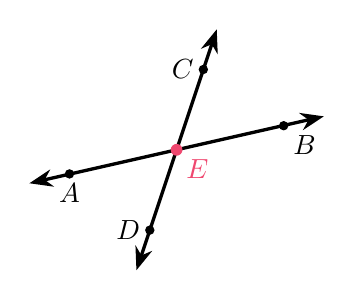
\begin{tikzpicture}[scale=0.85]\draw[very thick,{Stealth}-{Stealth}] (-2.2,-0.5)--(2.2,0.5); \draw[very thick,{Stealth}-{Stealth}] (-0.6,-1.8)--(0.6,1.8); \fill (-1.6,-0.36) circle(2pt) node[below]{$A$} (1.6,0.36) circle(2pt) node[below right]{$B$} (-0.4,-1.2) circle(2pt) node[left]{$D$} (0.4,1.2) circle(2pt) node[left]{$C$}; \fill[fmmistake] (0,0) circle(2.5pt) node[below right]{$E$};\end{tikzpicture}\end{minipage}\hfill
\begin{minipage}[c]{0.58\linewidth}\renewcommand{\arraystretch}{1.6}\begin{tabular}{@{}l l@{}}
$A$, $E$, $B$ are collinear & \fb[1.4cm]{can} assume\\
the two lines meet at $E$ & \fb[1.4cm]{can} assume\\
$\angle AEC = 90^\circ$ & \fb[1.4cm]{cannot} --- no \fb[3.4cm]{right-angle mark}\\
$AE = EB$ & \fb[1.4cm]{cannot} --- no \fb[2cm]{tick marks}\\
\end{tabular}\end{minipage}\end{watchme}

\vid{Marks tell you sizes}
\begin{keyidea}\begin{tabular}{@{}c c c@{}}
\tikz[baseline=0]{\draw[thick] (0,0)--(1,0) (0,0)--(0,1); \draw (0.2,0)--(0.2,0.2)--(0,0.2);} \quad \fb[2.2cm]{right angle} &
\tikz[baseline=0]{\draw[thick] (0,0.2)--(1.2,0.2); \draw (0.3,0.1)--(0.3,0.3) (0.9,0.1)--(0.9,0.3);} \quad \fb[2.4cm]{equal lengths} &
\tikz[baseline=0]{\draw[thick,-{Stealth}] (0,0.4)--(1.2,0.4); \draw[thick,-{Stealth}] (0,0)--(1.2,0); \draw[thick] (0.5,0.3)--(0.6,0.4)--(0.5,0.5) (0.5,-0.1)--(0.6,0)--(0.5,0.1);} \quad \fb[1.8cm]{parallel}\\
\end{tabular}\end{keyidea}

\vid{Watch out}
\begin{mistakebox}``It looks like it'' is \fb[1.2cm]{not} a reason. Only what is \fb[1.6cm]{drawn} (position) or \fb[1.6cm]{marked} (size) counts.\end{mistakebox}

\vid{Your turn}
\begin{yourturn}\begin{minipage}[c]{0.62\linewidth}Which can you assume?\par\vspace{1mm}
(a) $A$, $P$, $B$ are collinear \ \fb[1.2cm]{yes} --- drawn on one line\par\vspace{1mm}
(b) $PA = PB$ \ \fb[1.2cm]{yes} --- \fb[2cm]{tick marks}\par\vspace{1mm}
(c) the lines are perpendicular \ \fb[1.2cm]{no} --- no right-angle mark\end{minipage}\hfill
\begin{minipage}[c]{0.34\linewidth}\centering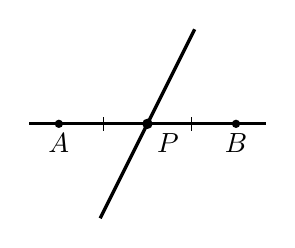
\begin{tikzpicture}[scale=0.75]\draw[very thick] (-2,0)--(2,0); \draw[very thick] (-0.8,-1.6)--(0.8,1.6); \fill (-1.5,0) circle(2pt) node[below]{$A$} (1.5,0) circle(2pt) node[below]{$B$} (0,0) circle(2.5pt) node[below right]{$P$}; \draw (-0.75,-0.12)--(-0.75,0.12) (0.75,-0.12)--(0.75,0.12);\end{tikzpicture}\end{minipage}\end{yourturn}

\begin{notebox}\textbf{Remember:}\quad Two points $\to$ one line; three noncollinear points $\to$ one plane.\quad Two lines meet in a point; two planes meet in a line.\quad Assume what is \textbf{drawn}, not sizes --- unless they are \textbf{marked}.\end{notebox}
\end{document}
